\documentclass[11pt,letterpaper]{article}

\usepackage[margin=1in]{geometry}
\usepackage[T1]{fontenc}
\usepackage[utf8]{inputenc}
\usepackage{newtxtext,newtxmath}
\usepackage{microtype}
\usepackage{setspace}
\usepackage{titlesec}
\usepackage{fancyhdr}
\usepackage{xcolor}
\usepackage{hyperref}
\usepackage{enumitem}
\usepackage{booktabs}
\usepackage{array}
\usepackage{longtable}
\usepackage{graphicx}
\graphicspath{{figures/}{../figures/}}

\hypersetup{
  colorlinks=true,
  linkcolor=black,
  citecolor=black,
  urlcolor=blue!50!black,
  pdftitle={STAT 248 Project Proposal},
  pdfauthor={Joshua Ren}
}

\setstretch{1.05}
\setlength{\parindent}{1em}
\setlength{\parskip}{0.25em}
\setlength{\headheight}{14pt}
\setlist[itemize]{leftmargin=1.4em, itemsep=0.2em, topsep=0.3em}
\urlstyle{same}

\titleformat{\section}
  {\large\bfseries}
  {\thesection.}
  {0.5em}
  {}
\titlespacing*{\section}{0pt}{1.0em}{0.4em}

\pagestyle{fancy}
\fancyhf{}
\lhead{\small STAT 248 Final Project Proposal}
\rhead{\small \thepage}
\renewcommand{\headrulewidth}{0.4pt}
\newcommand{\catmark}{\textsuperscript{\ensuremath{\dagger}}}

\newcommand{\ProposalTitle}{Temporal Structure and Forecasting of Hourly\\Bike-Sharing Demand in Washington, DC}
\newcommand{\ProposalDate}{April 15, 2026}
\newcommand{\CourseLine}{STAT 248: Analysis of Time Series}
\newcommand{\AuthorName}{Joshua Ren}
\newcommand{\AuthorSID}{3041881898}

\begin{document}

\begin{center}
  {\LARGE \bfseries \ProposalTitle \par}
  \vspace{1.1em}
  {\normalsize \textsc{\AuthorName} \quad {\normalfont |} \quad SID \AuthorSID \par}
\end{center}

\section{The Question}

Shared micromobility has become an important part of urban transportation in North America. According to the National Association of City Transportation Officials, shared micromobility systems recorded 157 million trips in the United States and Canada in 2023 \cite{nacto2024}. This growth has also created a greater need for effective short-term resource allocation. For station-based systems such as Capital Bikeshare, large hourly swings in usage directly affect bike availability \cite{capitalbikeshare2026}, making short-term demand forecasting operationally important.

This project studies hourly bike-sharing demand in Washington, DC. The main question is: \emph{what temporal structure characterizes hourly bike-sharing demand, and how well can short-term demand be forecast using historical usage and observed calendar and weather conditions?}

\section{Description of the Data}

The dataset comes from the Bike Sharing Dataset on Kaggle\footnote{The dataset can be found at \url{https://www.kaggle.com/datasets/lakshmi25npathi/bike-sharing-dataset}}. It contains two years of Capital Bikeshare usage data for Washington, D.C., together with weather and calendar information. The dataset includes files at both daily and hourly resolutions. In this project, the file \texttt{hour.csv} with hourly resolution is used to study demand patterns within and across days.

The hourly file contains 17,379 observations from January 1, 2011 through December 31, 2012. Each observation records the total number of bike rentals in a given hour, along with calendar and weather variables such as holiday status, temperature, and windspeed. The main series of interest is the aggregate hourly rental count, \texttt{cnt}. A detailed description of the variables is provided in Table \ref{tab:variable-definitions} in the Appendix.

A practical issue is that the raw file is missing 165 hourly timestamps, so a simple imputation procedure will be used to reconstruct a complete hourly series.

\begin{figure}[h]
  \centering
  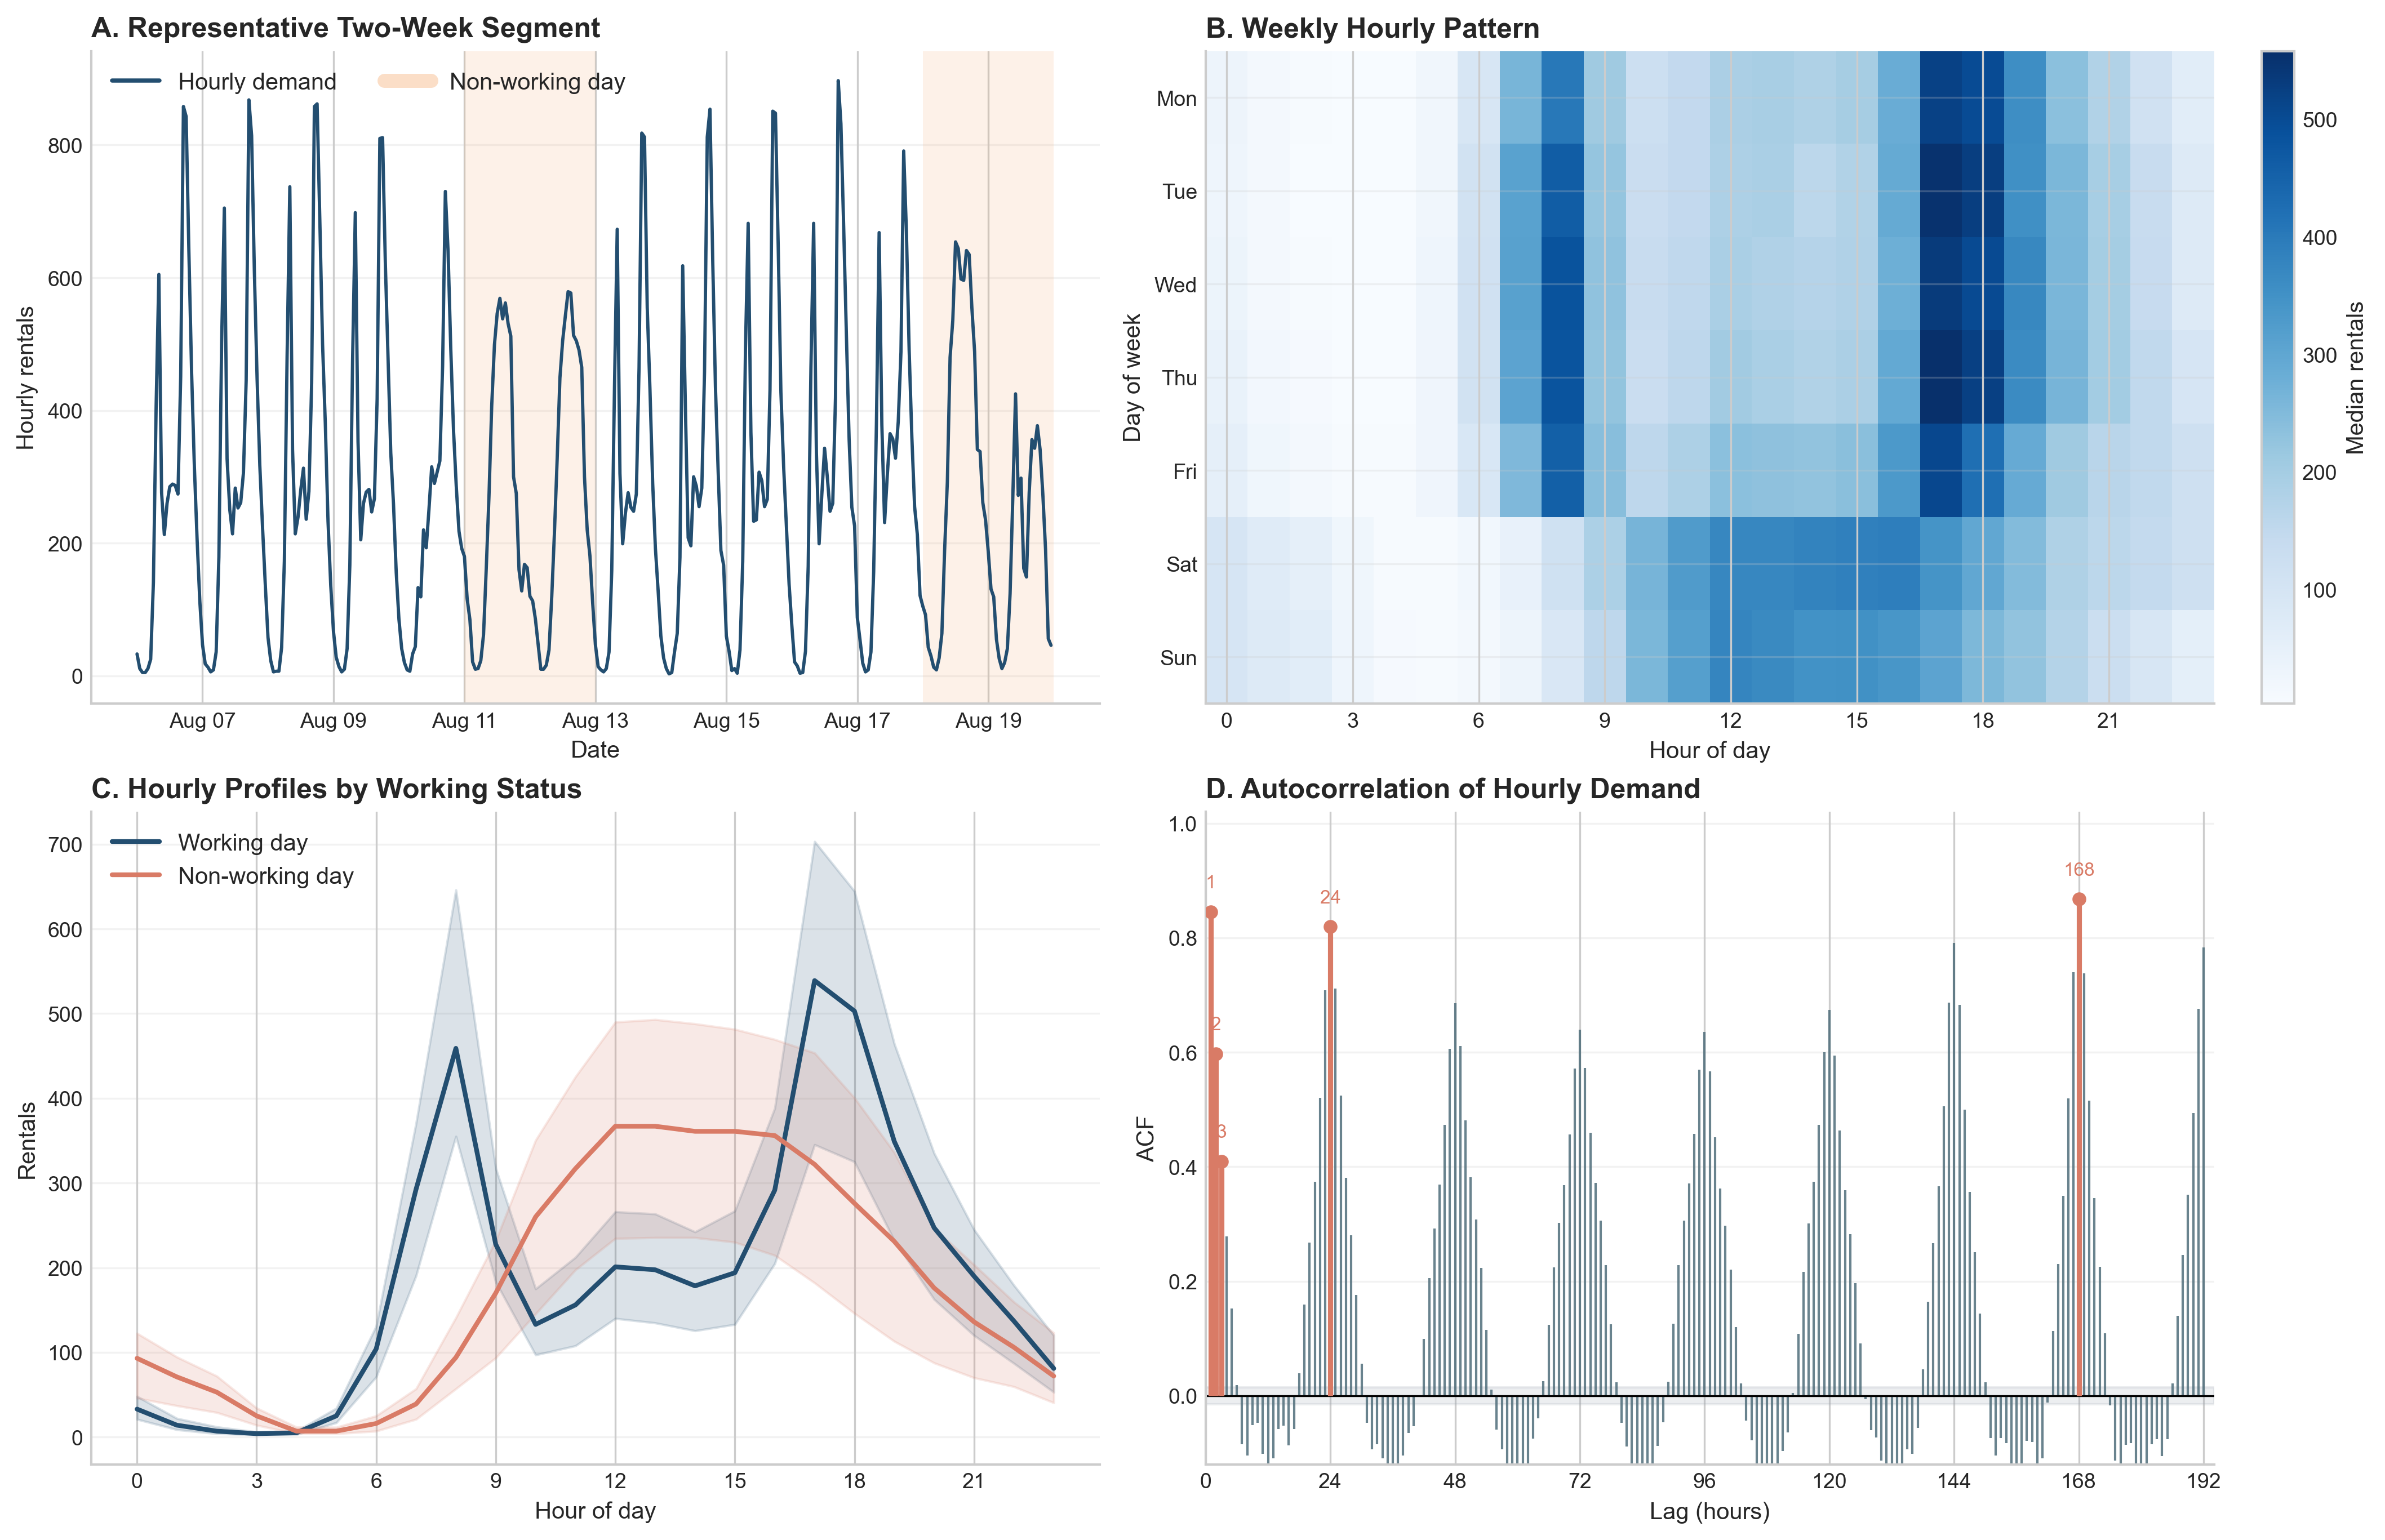
\includegraphics[width=0.9\textwidth]{hourly_demand_structure.png}
  \caption{Temporal structure of hourly bike-sharing demand}
  \label{fig:hourly-demand}
\end{figure}

\section{Why This Is a Time Series Problem}

In this bike-sharing context, current demand depends systematically on recent demand history. As shown in Figure \ref{fig:hourly-demand}, the hourly rental series clearly exhibits a daily cycle, short-run persistence, and differences between working days and non-working days. The autocorrelation function is also strong at lags 1, 2, 3, 24, and 168 hours, reflecting short-run persistence as well as daily and weekly repetition.

A model that treats the observations as independent would not capture the daily and weekly structure in the data. Since the goal of the project is to describe and predict this structure, time series methods are the natural framework for the analysis.



\section{Proposed Methods}

Three methods will be used for the analysis:

\textbf{1. ARIMA.} ARIMA will serve as the main classical benchmark since it relies only on the past values of the demand series. Because the hourly series shows a strong 24-hour cycle, I plan to difference it at lag 24 before fitting the model, so that the transformed series is closer to stationarity. ARIMA models of different orders will then be fitted to the transformed series. If time permits, I may briefly explore an ARIMAX-style extension with calendar and weather variables as additional work.

\textbf{2. Time-lagged regression.} I will then fit a time-lagged regression model that includes selected lag terms together with weather and calendar variables. Based on the ACF plot shown in Figure \ref{fig:hourly-demand}, the main lag terms will likely include \texttt{lag\_1}, \texttt{lag\_2}, \texttt{lag\_3}, \texttt{lag\_24}, and \texttt{lag\_168}. I may use ACF/PACF to determine the lag range. As additional work, I may consider ridge regularization to stabilize estimation.

\textbf{3. RNN/LSTM.} I will also consider recurrent neural network models, mainly an LSTM and possibly a simpler RNN. These models provide a more flexible way to learn nonlinear temporal relationships from past observations and external variables. Different input window lengths, such as 24, 72, and 168 hours, will be tested and compared.

These three methods address the same problem from different perspectives. For evaluation, I will use a time-ordered train-test split with a small gap between training and test periods to reduce leakage.

\section{Expected Outcomes}

Hourly bike demand is expected to be shaped by a combination of short-run persistence, daily and weekly repetition, and weather- or calendar-related variation. Under this expectation, time-lagged regression and the recurrent neural network models are likely to outperform the ARIMA benchmark. I also expect the LSTM to become more competitive as the input window becomes long enough to capture weekly structure.

A weaker result would be that weather and calendar variables add limited information beyond the demand series itself. It would suggest that most of the predictive information is already contained in the series' own temporal structure. Moreover, if the LSTM does not outperform lagged regression, one possible interpretation is that explicit lag terms and observed covariates already capture enough predictive information.


\newpage

\bibliographystyle{unsrt}
\IfFileExists{report.bib}{\bibliography{report}}{\bibliography{report/report}}

\appendix

\section{Definitions of Variables}

The table below summarizes the variables in \texttt{hour.csv}, which is the main dataset for this project.

\begingroup
\small
\setlength{\LTleft}{0pt}
\setlength{\LTright}{0pt}
\begin{longtable}{@{}>{\raggedright\arraybackslash}p{0.16\textwidth} >{\raggedright\arraybackslash}p{0.09\textwidth} >{\raggedright\arraybackslash}p{0.35\textwidth} >{\raggedright\arraybackslash}p{0.28\textwidth}@{}}
\caption{Variable definitions for the hourly bike sharing dataset\label{tab:variable-definitions}}\\
\toprule
Variable & Type & Description & Values/Units \\
\midrule
\endfirsthead

\toprule
Variable & Type & Description & Values/Units \\
\midrule
\endhead

\midrule
\multicolumn{4}{r}{\small\itshape Continued on next page} \\
\endfoot

\bottomrule
\endlastfoot

\multicolumn{4}{@{}l}{\textbf{Time and Calendar Variables}} \\
\addlinespace[0.2em]
instant & int & Record index in the original file & 1--17,379 \\
dteday & date & Calendar date of the observation & YYYY-MM-DD \\
season\catmark & int & Season indicator & 1: spring, 2: summer, 3: fall, 4: winter \\
yr\catmark & int & Year indicator & 0: 2011, 1: 2012 \\
mnth\catmark & int & Month of year & 1--12 \\
hr\catmark & int & Hour of day & 0--23 \\
holiday\catmark & int & Holiday indicator & 1: yes, 0: no \\
weekday\catmark & int & Day of week & 0--6 \\
workingday\catmark & int & Working-day indicator & 1: yes, 0: no \\
\addlinespace[1em]

\multicolumn{4}{@{}l}{\textbf{Weather Variables}} \\
\addlinespace[0.2em]
weathersit\catmark & int & Categorical weather condition & 1: clear, 2: mist/cloudy, 3: light snow/rain, 4: heavy rain/snow \\
temp & float & Normalized temperature & scaled to $[0,1]$ in source data \\
atemp & float & Normalized feeling temperature & scaled to $[0,1]$ in source data \\
hum & float & Normalized humidity & scaled to $[0,1]$ in source data \\
windspeed & float & Normalized wind speed & scaled to $[0,1]$ in source data \\
\addlinespace[1em]

\multicolumn{4}{@{}l}{\textbf{Demand Variables}} \\
\addlinespace[0.2em]
casual & int & Count of non-registered users & hourly rental count \\
registered & int & Count of registered users & hourly rental count \\
cnt & int & Total bike rental demand & hourly rental count \\
\addlinespace[1em]
\end{longtable}
\noindent\footnotesize \catmark\ indicates categorical variables, including binary indicators and ordered calendar codes.
\endgroup

In the analysis, \texttt{cnt} is the response variable. The variables \texttt{casual} and \texttt{registered} will not be used as predictors because they sum to \texttt{cnt}.

\end{document}
